%----------------------------------------------------------------------------------------
%	PACKAGES AND DOCUMENT CONFIGURATIONS
%----------------------------------------------------------------------------------------

\documentclass{article}

\usepackage{graphicx} % Required for the inclusion of images
\usepackage{subfigure} % Required for the inclusion of images
\usepackage{natbib} % Required to change bibliography style to APA
\usepackage{amsmath} % Required for some math elements 

\usepackage{listings}
\usepackage{color}
\lstset{breaklines=true}

\usepackage{listings}
\usepackage{xcolor}
\usepackage{indentfirst}
\setlength{\parindent}{2em}


% 定义可能使用到的颜色
\definecolor{CPPLight}  {HTML} {686868}
\definecolor{CPPSteel}  {HTML} {888888}
\definecolor{CPPDark}   {HTML} {262626}
\definecolor{CPPBlue}   {HTML} {4172A3}
\definecolor{CPPGreen}  {HTML} {487818}
\definecolor{CPPBrown}  {HTML} {A07040}
\definecolor{CPPRed}    {HTML} {AD4D3A}
\definecolor{CPPViolet} {HTML} {7040A0}
\definecolor{CPPGray}  {HTML} {B8B8B8}
\lstset{
    columns=fixed,       
    numbers=left,                                        % 在左侧显示行号
    frame=none,                                          % 不显示背景边框
    backgroundcolor=\color[RGB]{245,245,244},            % 设定背景颜色
    keywordstyle=\color[RGB]{40,40,255},                 % 设定关键字颜色
    numberstyle=\footnotesize\color{darkgray},           % 设定行号格式
    commentstyle=\it\color[RGB]{0,96,96},                % 设置代码注释的格式
    stringstyle=\rmfamily\slshape\color[RGB]{128,0,0},   % 设置字符串格式
    showstringspaces=false,                              % 不显示字符串中的空格
    language=c,                                        % 设置语言
    morekeywords={alignas,continute,friend,register,true,alignof,decltype,goto,
    reinterpret_cast,try,asm,defult,if,return,typedef,auto,delete,inline,short,
    typeid,bool,do,int,signed,typename,break,double,long,sizeof,union,case,
    dynamic_cast,mutable,static,unsigned,catch,else,namespace,static_assert,using,
    char,enum,new,static_cast,virtual,char16_t,char32_t,explict,noexcept,struct,
    void,export,nullptr,switch,volatile,class,extern,operator,template,wchar_t,
    const,false,private,this,while,constexpr,float,protected,thread_local,
    const_cast,for,public,throw,std},
}


%\usepackage{times} % Uncomment to use the Times New Roman font

%----------------------------------------------------------------------------------------
%	DOCUMENT INFORMATION
%----------------------------------------------------------------------------------------

\title{\textbf{Project 2:  Understanding Cache Memories}} % Title

\author{Jingwei Xi, 517030910116, jingweixi@sjtu.edu.cn } % Author name and email

\date{\today} % Date for the report

\begin{document}

\maketitle % Insert the title, author and date

\section{Introduction}


In this lab, I write two programs for two parts. In the first part, I write a program to simulate the hit, miss and evict behaviors of an LRU cache memory. In the program, I use array to be the data structure for cache. In the second part, I write a program to optimize cache performance for matrix transpose function.

\section{Experiments}

\subsection{Part A}

\subsubsection{Analysis}


The task for part A is to simulate the behavior of a cache with arbitrary size and associativity on a valgrind trace file. To complete this task, I use array to simulate the cache.

In each element of array, I use three variables. First is valid bit, which indicate whether the data of block in cache is valid. The second variable is tag, which is used to check whether block is in the cache. The third one is the timeRef, which stores the time that the block recently be accessed. 

I use the LRU (least-recently used) replacement policy when choosing which cache line to evict. For each data access, there will be three situation: 

a. The data block is in the cache. 

b. The data block is not in the cache but there is empty line in the set. It will put the block into empty line.

 c. The data block is not in the cache and there is not empty line in the set. It will evict the line with minimum timeRef number, which indicate it has not been accessed for a long time.

\subsubsection{Code}

\begin{lstlisting}[title=csim.c, frame=shadowbox]
//517030910116    Jingwei Xi
//email: jingweixi@sjtu.edu.cn
//This is the program for simulating the behavior of a cache
#include "cachelab.h"
#include <getopt.h>
#include <stdio.h>
#include <stdlib.h>
#include <math.h>
#include <limits.h>
#include <memory.h>

typedef struct{
    int valid;
    long unsigned int tag;
    int timeRef;
}line;   // The line in cache array

typedef struct{
    int helpFlag;           //-h 
    int verboseFlag;        //-v
    int setBit;             //-s 
    int linePerSet;         //-e
    int blockBit;           //-b
    char *fileName;         //-t
}argument;     //The parameters of instruction

line *cache;
argument mainArg;

int setCount;
int blockSize;
int cacheSize;
int hit;
int miss;
int eviction;
int timeClock = 0;

void printHelp(){
    printf("Usage: ./csim-wrc [-hv] -s <s> -E <E> -b <b> -t <tracefile>\n");
    printf("-h: Optional help flag that prints usage info\n");
    printf("-v: Optional verbose flag that displays trace info\n");
    printf("-s <s>: Number of set index bits (S = 2^s is the number of sets)\n");
    printf("-E <E>: Associativity (number of lines per set)\n");
    printf("-b <b>: Number of block bits (B = 2^b is the block size)\n");
    printf("-t <tracefile>: Name of the valgrind trace to replay\n");
}

void initMainArg(){
    mainArg.helpFlag = 0;
    mainArg.verboseFlag = 0;
    mainArg.setBit = 0;
    mainArg.linePerSet = 0;
    mainArg.blockBit = 0;
    mainArg.fileName = NULL;
}

void cacheAccess(char type, long unsigned int addr, int size){
    int hitFlag = 0, hitId = -1, emptyLine = -1, minTime = INT_MAX, evicId;
    int setIndex = 0;
    int dataTag;
    int i;
    
    //Address: |tag|setIndex|block_offset|
    setIndex = (addr / (blockSize)) % (setCount);
    dataTag = addr / (blockSize * setCount);

    for(i = setIndex * mainArg.linePerSet; i < (setIndex + 1) * mainArg.linePerSet; i++){
        //Hit
        if(cache[i].tag == dataTag){
            hitFlag = 1;
            hitId = i;
            break;
        }
        //Record the empty line id
        if(cache[i].valid == 0 && emptyLine == -1){ 
            emptyLine = i;
        }
        //Find the block line with the minimum timeRef number
        if(cache[i].timeRef < minTime){  
            minTime = cache[i].timeRef;
            evicId = i;
        }
    }

    if (mainArg.verboseFlag){
        printf("%c %lx,%x ",type,addr,size);
    }
    if(hitFlag == 1){    //Hit
        cache[hitId].timeRef = timeClock;
        hit++;
        if(type == 'M'){
            hit++;
        }
        if(mainArg.verboseFlag){
            if(type == 'S' || type == 'L'){
                printf("hit\n");
            }
            else{
                printf("hit hit\n");
            }
        }
        
    }
    else{
        if(emptyLine != -1){//Miss but there is empty line
            cache[emptyLine].valid = 1;
            cache[emptyLine].tag = dataTag;
            cache[emptyLine].timeRef = timeClock;
            miss++;
            if(type == 'M'){
                hit++;
            }
            if(mainArg.verboseFlag){
                if(type == 'S' || type == 'L'){
                    printf("miss\n");
                }
                else{
                    printf("miss hit\n");
                }
            }
        }
        else{    //Miss and no empty line, need to evict
            cache[evicId].valid = 1;
            cache[evicId].tag = dataTag;
            cache[evicId].timeRef = timeClock;
            miss++;
            eviction++;
            if(type == 'M'){
                hit++;
            }
            if(mainArg.verboseFlag){
                if(type == 'S' || type == 'L'){
                    printf("miss evition\n");
                }
                else{
                    printf("miss eviction hit\n");
                }
            }           
        }
    }
}

int main(int argc, char* argv[])
{
    int opt;
    int i;
    char type;
    int size;
    long unsigned int addr;

    initMainArg();//init each variable in argument struct 

    opt = getopt(argc, argv, "s:E:b:t:hv");
    if(opt == -1){     //Invalid arguments
        printHelp();
        return -1;
    }
    while(opt != -1) {
        switch(opt){
            case 'v':
                mainArg.verboseFlag = 1; /* true */
                break;          
            case 's':
                mainArg.setBit = atoi(optarg);
                break;               
            case 'E':
                mainArg.linePerSet = atoi(optarg);
                break;                 
            case 'b':
                mainArg.blockBit = atoi(optarg);
                break;            
            case 't':   
                mainArg.fileName = optarg;
                break;
            default:
                printHelp();
                break;
        }     
        opt = getopt(argc, argv, "s:E:b:t:hv");
    }

    setCount = 1 << (mainArg.setBit);
    blockSize = 1 << (mainArg.blockBit);

    FILE *file = fopen(mainArg.fileName, "r");
    if (file == NULL){   //Error: File not found
	printf("File not found.");
	return -1;
    }

    cache = (line *) malloc(setCount * mainArg.linePerSet * sizeof(line));
	if (cache == NULL){   //Error: Cache space allocated failed
	    printf("Fail to allocate cache.");
	    return -1;
	}

    cacheSize = setCount * mainArg.linePerSet;
    //Initialize the cache
    for (i = 0; i < cacheSize; i++) {
	cache[i].valid = 0;
	cache[i].timeRef = 0;
        cache[i].tag = -1;
    }

    while (!feof(file)){
	int tmp = fscanf(file, " %c %lx,%x", &type, &addr, &size);
	if (tmp != 3) continue;
	if (type == 'I') continue;
	cacheAccess(type, addr, size);
	timeClock++;
    }

    free(cache);    //Free the cache space malloced
    cache = NULL;
    printSummary(hit, miss, eviction);
    return 0;
}

\end{lstlisting}


\subsubsection{Evaluation}

Here is the result. \\

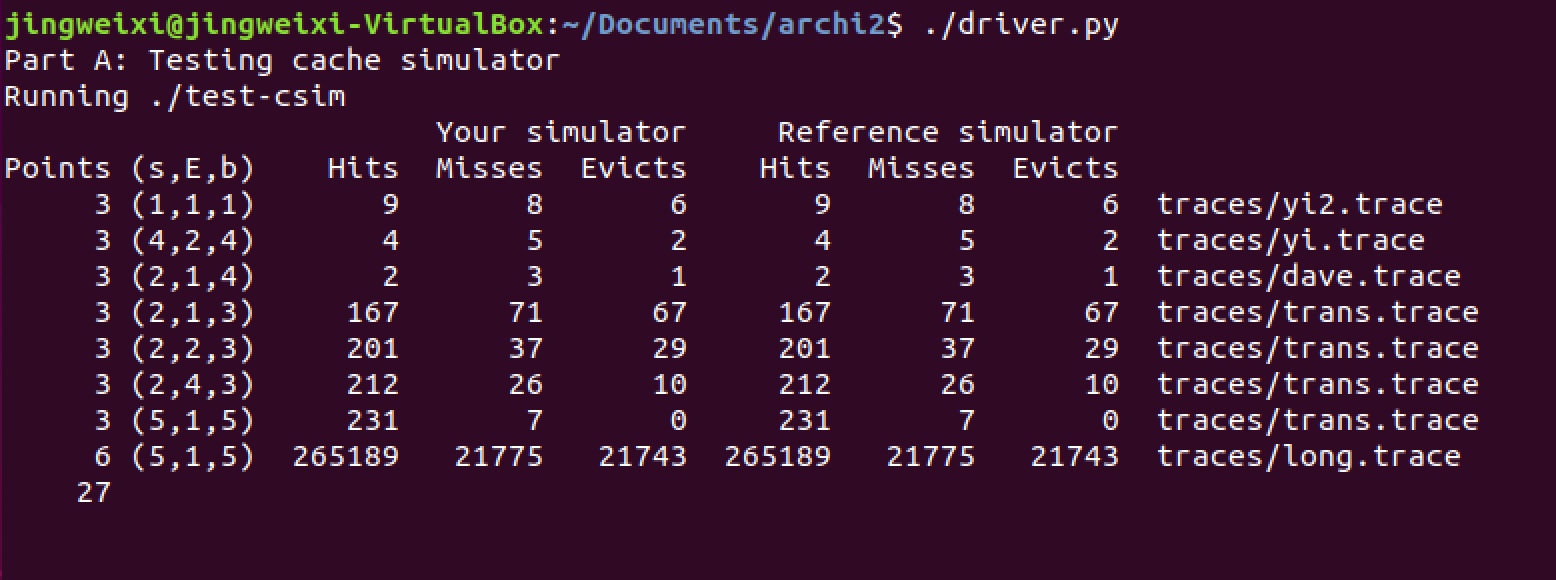
\includegraphics[scale=0.43]{1.png}

\subsection{Part B}

\subsubsection{Analysis}

The task of part B is to write a transpose function that causes as few cache misses as possible. 

For 32x32 matrix, each element in matrix with int type use 4 bytes. As our block size is 32 bytes, we have 
8 elements in one block. For each line in matrix, it can be placed in 4 blocks and the cache will save 8 lines of matrix at one time.

The cache block distribution of matrix elements is showed in the picture.

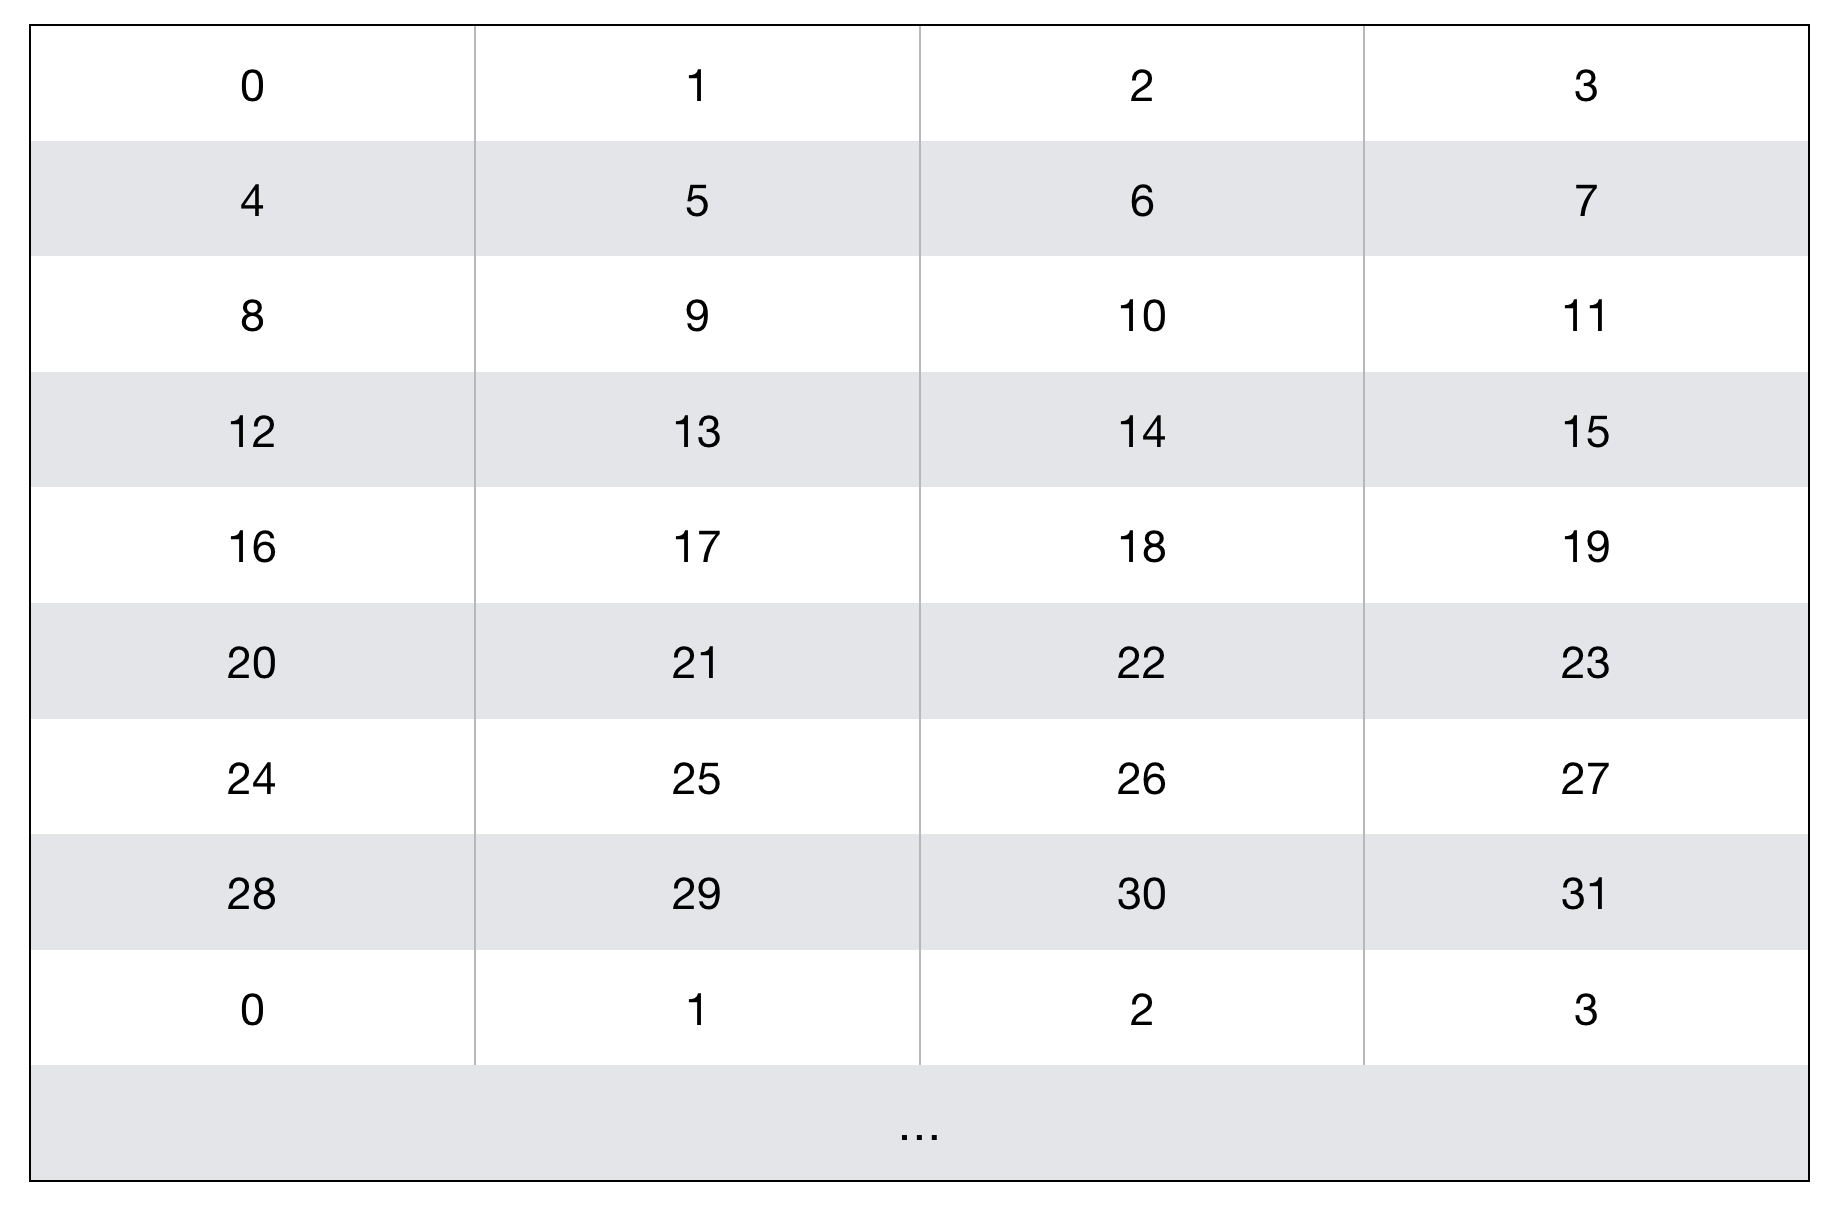
\includegraphics[scale=0.35]{2.png}

From the picture, we can see that we can deal with 8x8 matrix each time with few conflict misses because all matrix element are in the cache.

And for elements like A[i][i], the lines we’ll use in matrix A and matrix B are mapped to the same cache line, which will generate unnecessary conflict misses. So we will use a temporary variant to store the value temporarily and transfer to matrix B later.

For 64x64 matrix, the situation is different from 32x32 before. 

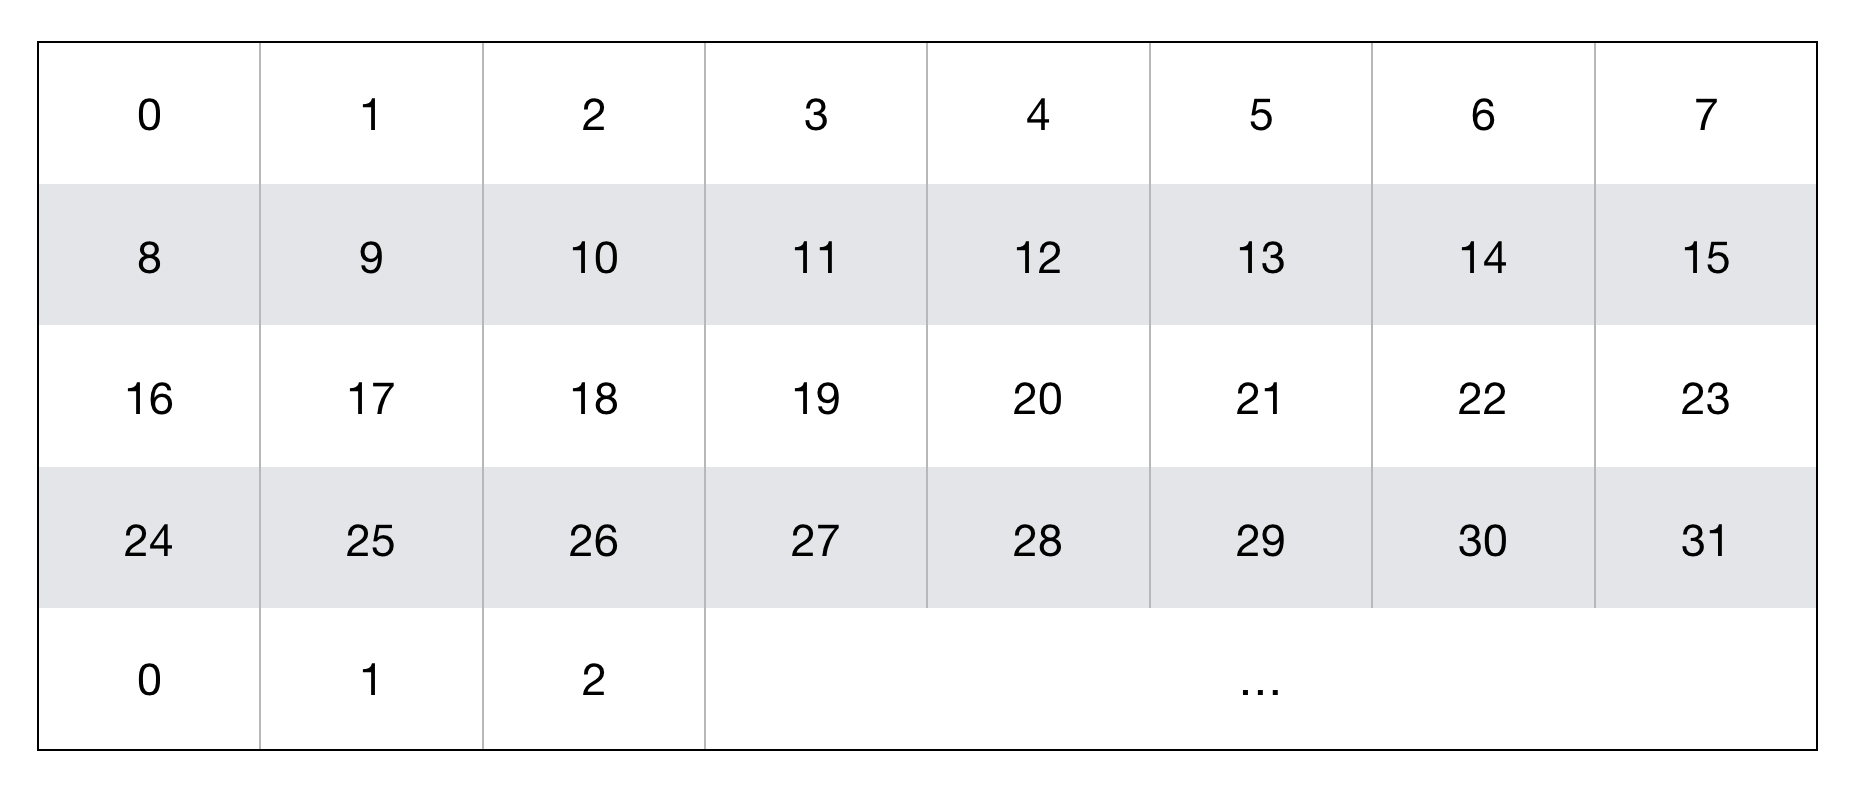
\includegraphics[scale=0.35]{3.png}

From the picture we can see that each line in matrix can be placed in 8 blocks and the cache will save 4 lines of matrix at one time. So only 4*4 matrix can be placed in cache at one time. If we transpose 4*4 matrix at on time, it can have little miss but it will waste a lot of space in cache line. The algorithm I  developed will use 8*8 matrix which can fully use of cache line and have a good performance.

Firstly, there is matrix A and matrix B, and both of them are 8x8. I divide A and B into four 4x4 matrices: A, B, C, D. At this time, the matrix B is empty.

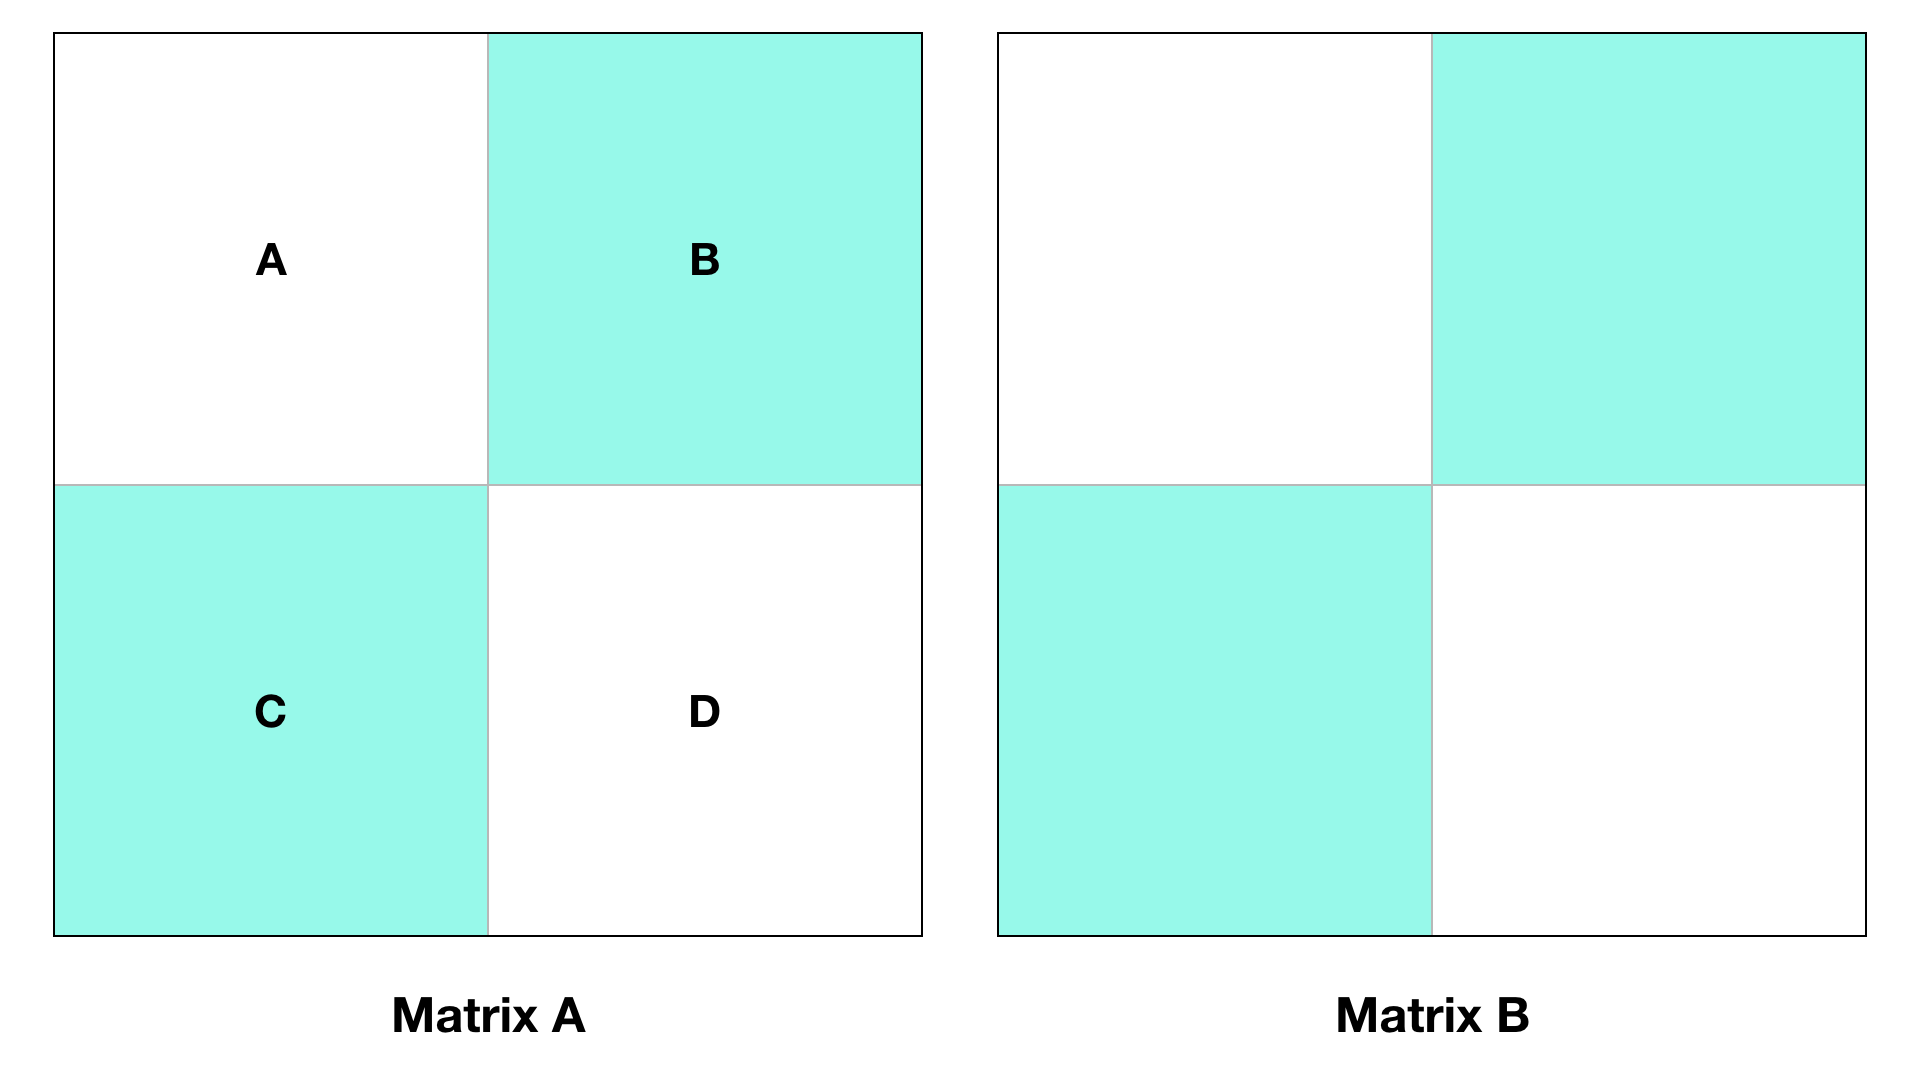
\includegraphics[scale=0.35]{4.png}

Secondly, I put AT andBT into matrix B. Because four lines of matrix can be saved in cache at the same time, we can handle  A and B at the same time with little misses.

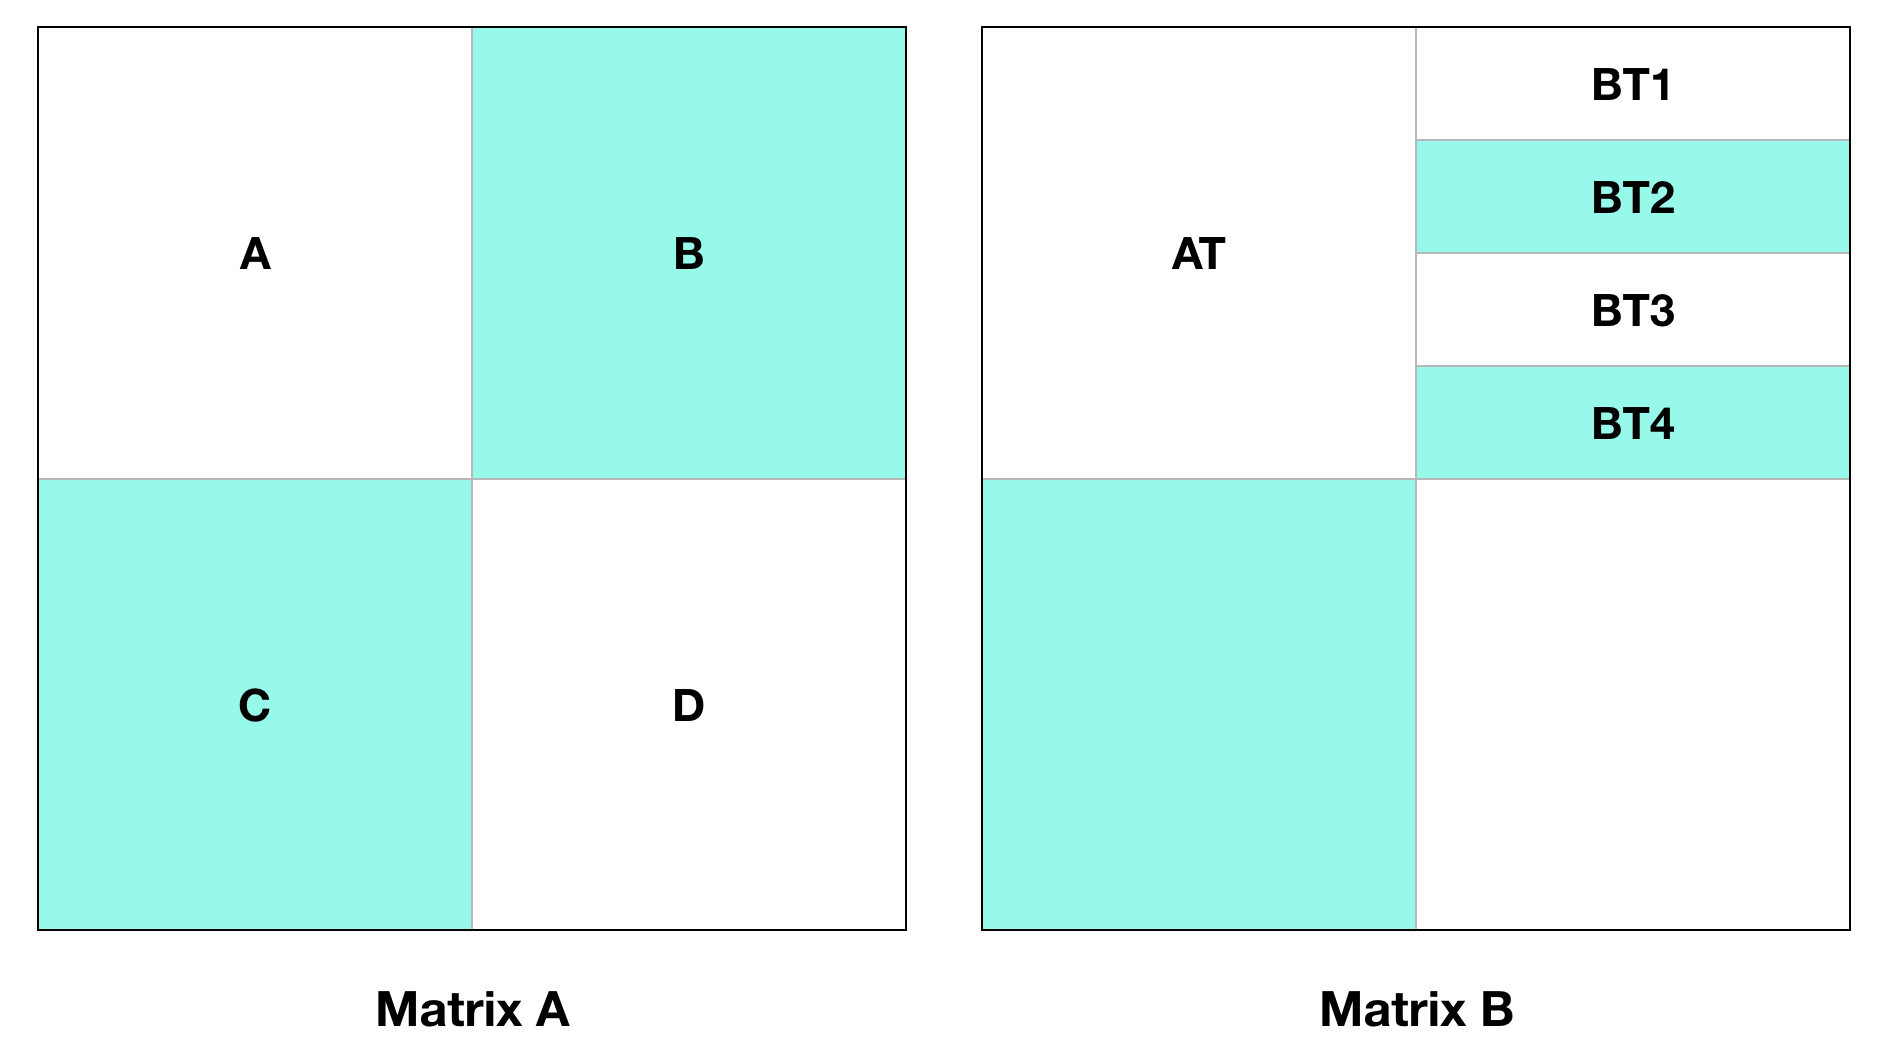
\includegraphics[scale=0.35]{5.png}

Thirdly, I put BT into right place by row. And then I put CT to right place by column. The transfer algorithm is showed in the picture.

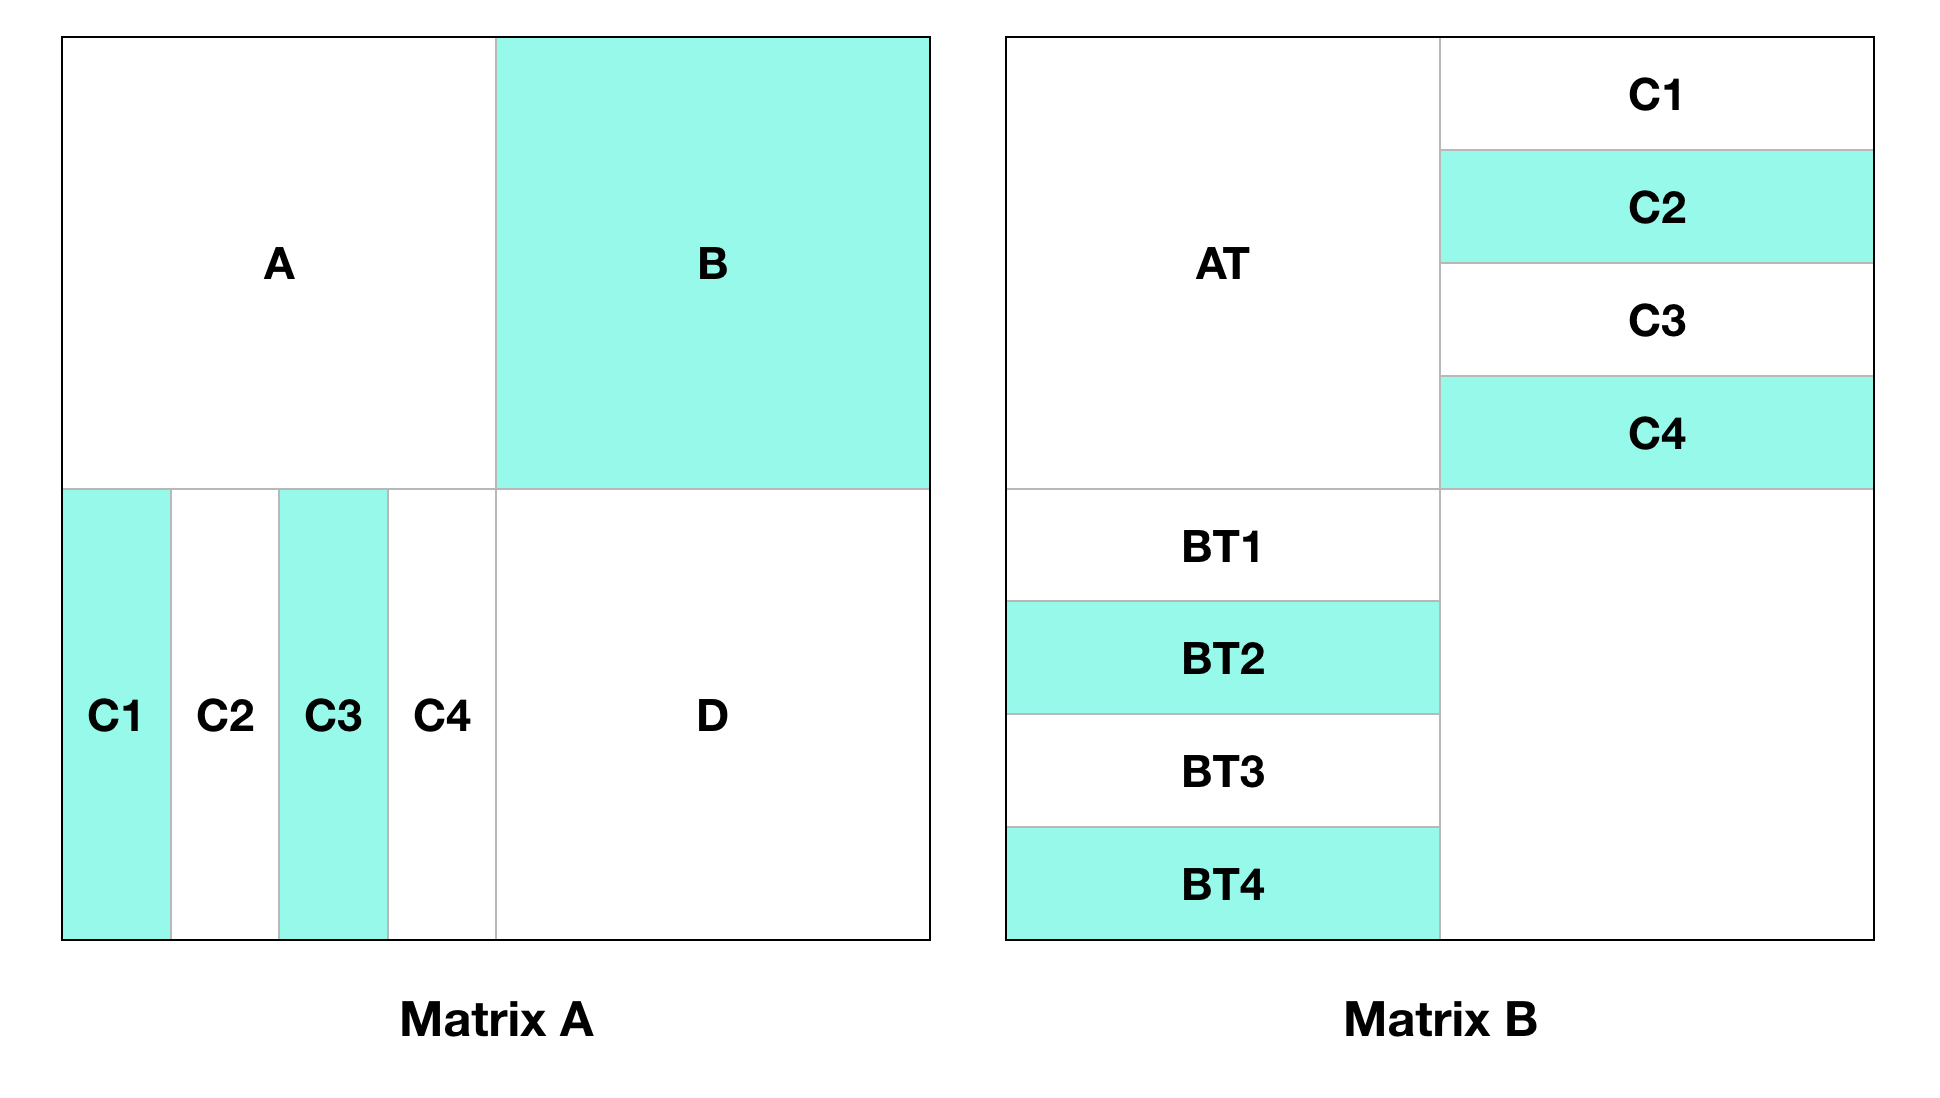
\includegraphics[scale=0.35]{6.png}

At last, I put DT to matrix B.

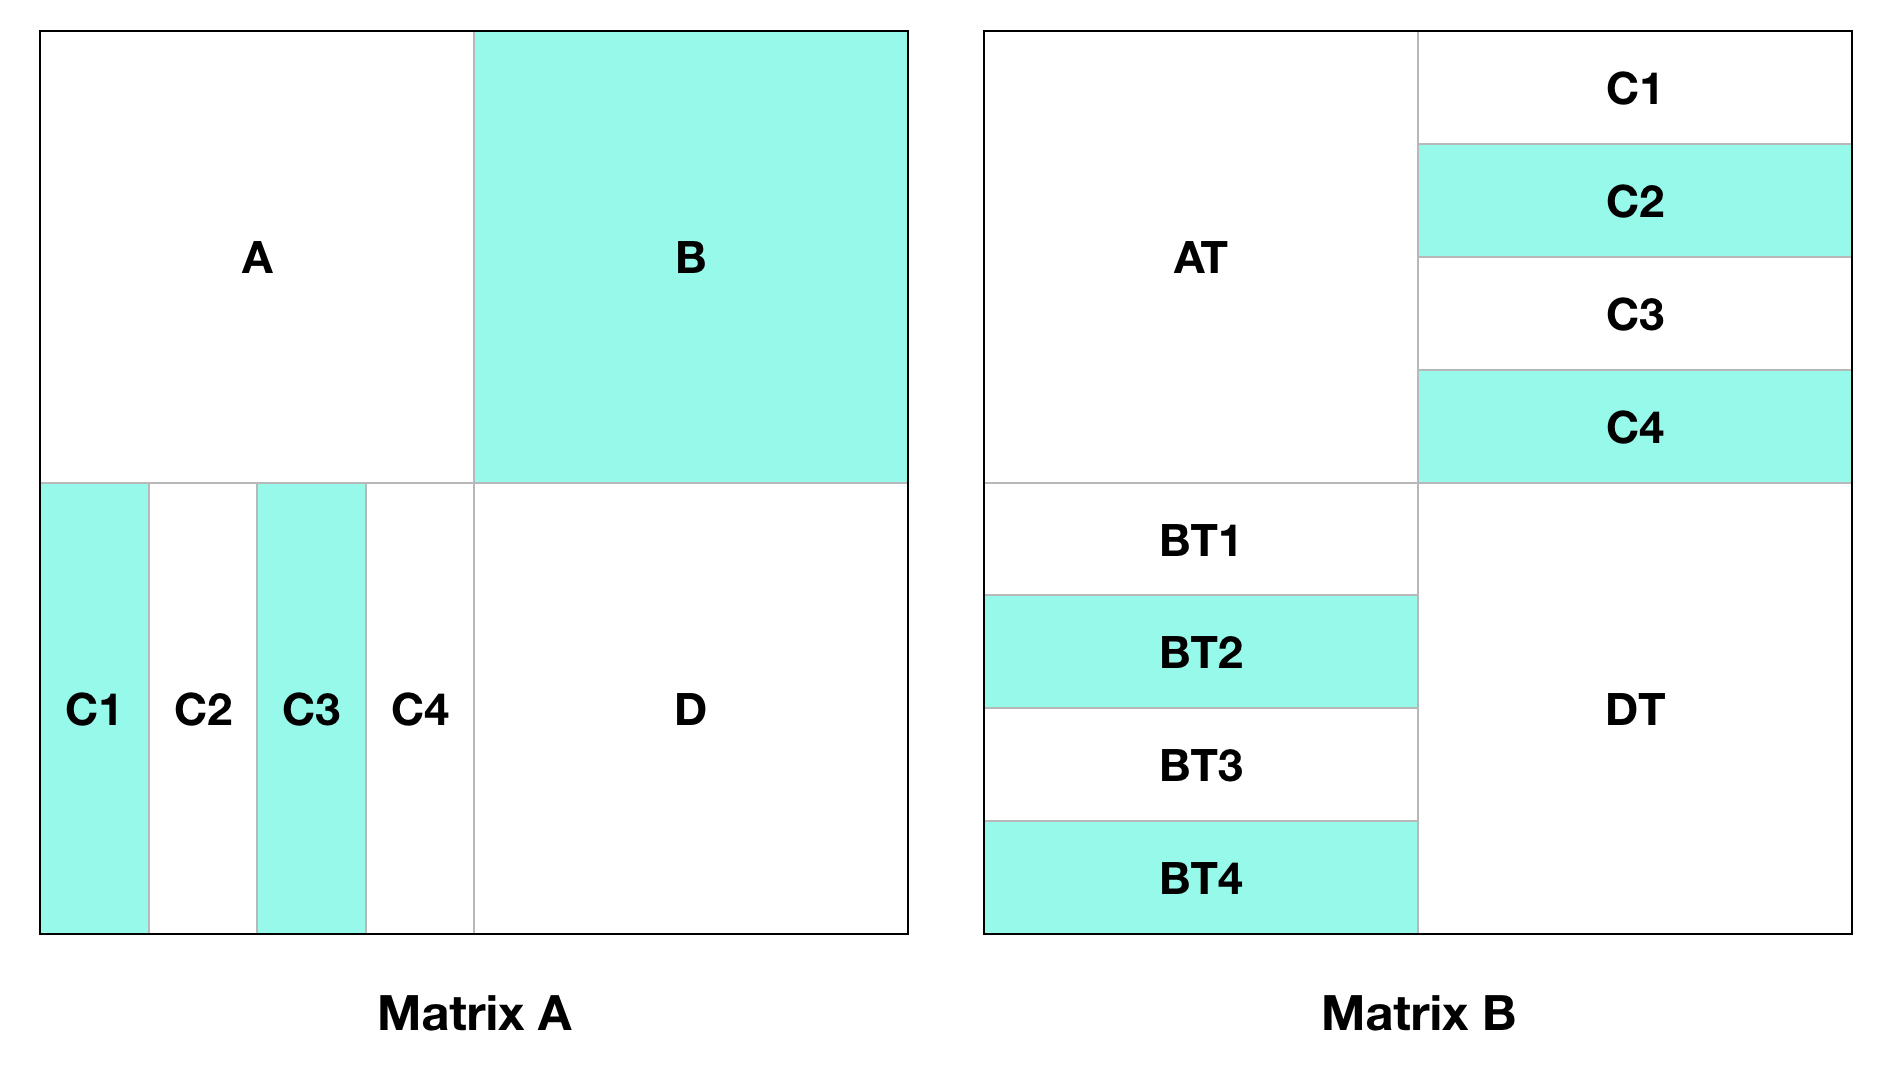
\includegraphics[scale=0.35]{7.png}

Even though I can not modify matrix A, I can matrix B at any time. When I transpose B and C in matrix A, I use empty space in B to temporarily save BT, which will reduce many conflict misses.

For 61x67 matrix, I can not calculate the best unit size for matrix transposition. So I just test different unit sizes to handle it and I find that use 16x16 size matrix as the unit will meet the requirement.
\subsubsection{Code}

\begin{lstlisting}[title=trans.c, frame=shadowbox]
//517030910116    Jingwei Xi
//email: jingweixi@sjtu.edu.cn
//This is the program for matrix transpose function
/* 
 * trans.c - Matrix transpose B = A^T
 *
 * Each transpose function must have a prototype of the form:
 * void trans(int M, int N, int A[N][M], int B[M][N]);
 *
 * A transpose function is evaluated by counting the number of misses
 * on a 1KB direct mapped cache with a block size of 32 bytes.
 */ 

#include <stdio.h>
#include "cachelab.h"

int is_transpose(int M, int N, int A[N][M], int B[M][N]);

/* 
 * transpose_submit - This is the solution transpose function that you
 *     will be graded on for Part B of the assignment. Do not change
 *     the description string "Transpose submission", as the driver
 *     searches for that string to identify the transpose function to
 *     be graded. 
 */
char transpose_submit_desc[] = "Transpose submission";
void transpose_submit(int M, int N, int A[N][M], int B[M][N])
{
    int i, j, m, n;
    int a1, a2, a3, a4, a5, a6, a7, a8;
    if(N == 32 && M == 32){   // Matrix 32x32
        for(i = 0; i < 4; i++){
            for(j = 0; j < 4; j++){
                for(m = 0; m < 8; m++){
                    for(n = 0; n < 8; n++){
                        //For A[k][k], handle it later
                        if(i * 8 + m == j * 8 + n){
                            a1 = i * 8 + m;
                            a2 = A[i * 8 + m][j * 8 + n];
                            continue;
                        }
                        B[j * 8 + n][i * 8 + m] = A[i * 8 + m][j * 8 + n];
                    }
                    if(i == j){
                        //Handle the A[k][k]
                        B[a1][a1] = a2;  
                    }
                }
            }
        }
        return;
    }

    if(N == 64 && M == 64){  //Matrix 64x64
        
        for(i = 0; i < 8; i++){
            for(j = 0; j < 8; j++){
                //Transpose A,B to AT, BT
                for(m = 0; m < 4; m++){
                    a1 = A[i * 8 + m][j * 8]; 
                    a2 = A[j * 8 + m][j * 8 + 1];
                    a3 = A[j * 8 + m][j * 8 + 2]; 
                    a4 = A[j * 8 + m][j * 8 + 3];
                    a5 = A[j * 8 + m][j * 8 + 4]; 
                    a6 = A[j * 8 + m][j * 8 + 5];
                    a7 = A[j * 8 + m][j * 8 + 6]; 
                    a8 = A[j * 8 + m][j * 8 + 7];

                    B[j * 8][i * 8 + m] = a1;
                    B[j * 8][i * 8 + m + 4] = a5;
                    B[j * 8 + 1][i * 8 + m] = a2;
                    B[j * 8 + 1][i * 8 + m + 4] = a6;
                    B[j * 8 + 2][i * 8 + m] = a3;
                    B[j * 8 + 2][i * 8 + m + 4] = a7;
                    B[j * 8 + 3][i * 8 + m] = a4;
                    B[j * 8 + 3][i * 8 + m + 4] = a8;

                }
                //Transfer BT and CT to right place 
                for(m = 0; m < 4; m++){
                    a1 = B[j * 8 + m][i * 8 + 4];
                    a2 = B[j * 8 + m][i * 8 + 5];
                    a3 = B[j * 8 + m][i * 8 + 6];
                    a4 = B[j * 8 + m][i * 8 + 7];
                    a5 = A[i * 8 + 4][j * 8 + m];
                    a6 = A[i * 8 + 5][j * 8 + m];
                    a7 = A[i * 8 + 6][j * 8 + m];
                    a8 = A[i * 8 + 7][j * 8 + m];
                    
                    B[j * 8 + m][i * 8 + 4] = a5;
                    B[j * 8 + m][i * 8 + 5] = a6;
                    B[j * 8 + m][i * 8 + 6] = a7;
                    B[j * 8 + m][i * 8 + 7] = a8;
                    B[j * 8 + m + 4][i * 8] = a1;
                    B[j * 8 + m + 4][i * 8 + 1] = a2;
                    B[j * 8 + m + 4][i * 8 + 2] = a3;
                    B[j * 8 + m + 4][i * 8 + 3] = a4;
                }
                //Transpose D to DT
                for(m = 0; m < 4; m++){
                    a1 = A[i * 8 + 4 + m][j * 8 + 4];
                    a2 = A[i * 8 + 4 + m][j * 8 + 5];
                    a3 = A[i * 8 + 4 + m][j * 8 + 6];
                    a4 = A[i * 8 + 4 + m][j * 8 + 7];

                    B[j * 8 + 4][i * 8 + m + 4] = a1;
                    B[j * 8 + 5][i * 8 + m + 4] = a2;
                    B[j * 8 + 6][i * 8 + m + 4] = a3;
                    B[j * 8 + 7][i * 8 + m + 4] = a4;  
                }
            }
        }
        return;
    }
    //Matrix 61x67, use unit 16x16
    for(i = 0; i < 16; i++){
        for(j = 0; j < 16; j++){
            for(m = 0; m < 16 && m < N; m++){
                for(n = 0; n < 16 && n < M; n++){
                    B[j * 8 + n][i * 8 + m] = A[i * 8 + m][j * 8 + n];
                }
            }
        }
    }
}

/* 
 * You can define additional transpose functions below. We've defined
 * a simple one below to help you get started. 
 */ 

/* 
 * trans - A simple baseline transpose function, not optimized for the cache.
 */
char trans_desc[] = "Simple row-wise scan transpose";
void trans(int M, int N, int A[N][M], int B[M][N])
{
    int i, j, tmp;

    for (i = 0; i < N; i++) {
        for (j = 0; j < M; j++) {
            tmp = A[i][j];
            B[j][i] = tmp;
        }
    }    

}

/*
 * registerFunctions - This function registers your transpose
 *     functions with the driver.  At runtime, the driver will
 *     evaluate each of the registered functions and summarize their
 *     performance. This is a handy way to experiment with different
 *     transpose strategies.
 */
void registerFunctions()
{
    /* Register your solution function */
    registerTransFunction(transpose_submit, transpose_submit_desc); 

    /* Register any additional transpose functions */
    registerTransFunction(trans, trans_desc); 

}

/* 
 * is_transpose - This helper function checks if B is the transpose of
 *     A. You can check the correctness of your transpose by calling
 *     it before returning from the transpose function.
 */
int is_transpose(int M, int N, int A[N][M], int B[M][N])
{
    int i, j;

    for (i = 0; i < N; i++) {
        for (j = 0; j < M; ++j) {
            if (A[i][j] != B[j][i]) {
                return 0;
            }
        }
    }
    return 1;
}



\end{lstlisting}
\subsubsection{Evaluation}

Here are the results and correctness of my program.\\


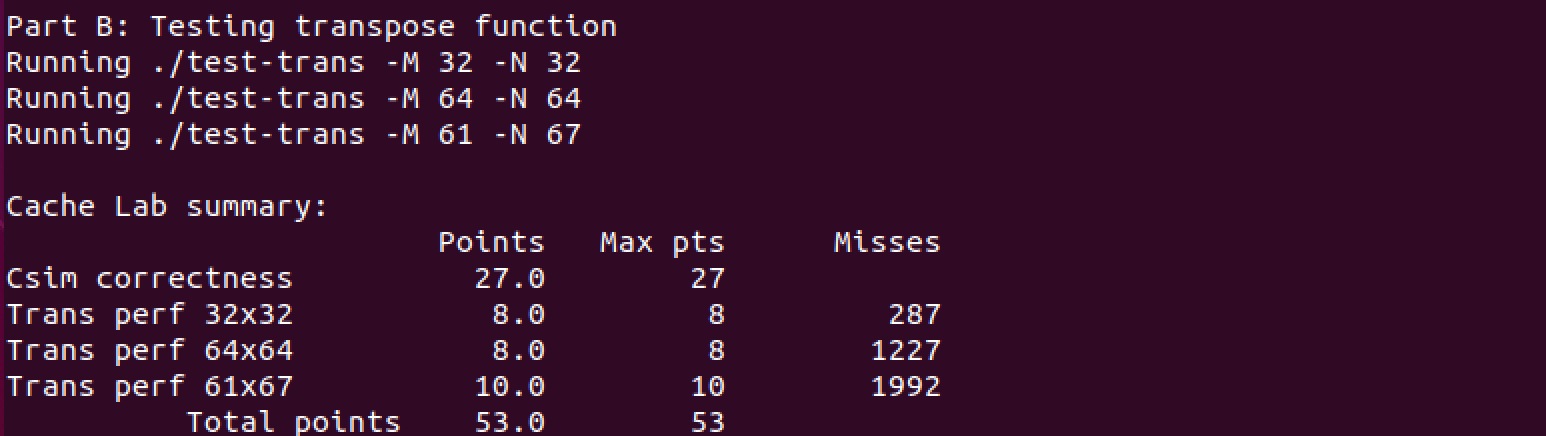
\includegraphics[scale=0.43]{8.png}


\section{Conclusion}

\subsection{Problems}

In part A, I met the problem that I didn't not know how to get the arguments of command line with uncertain number of arguments. With the help of partner and some technology blogs on the internet, I learned how to use the function getopt() to get the argument value.

The most difficult obstacle I met in this project is in part B. For transposition of matrix 64x64, the optimization of matrix 32x32 and 61x67 are both not work well. I think a lot of ideas to optimize on handling in a unit matrix of 4x4, but they all did not meet requirements. After learning some best idea on the internet and discussing with partners , I solve this problem by temporarily using the empty space in matrix B.

\subsection{Achievements}

In part A, my program takes the same command line arguments and produces the identical output as the reference simulator. In part B, the algorithm I used has a good performance that misses of cache are all meet requirements.

In this project, I discuss the algorithm in part B with my partner several times. During the discuss, we all think about how to improve  performance of our program and talk about ideas with others. I make a good progress during the time as we optimize our algorithm.

At the same time, I learned a lot of knowledge of cache and make a deep comprehension of cache LRU algorithm. In addition, with the practice in part B, l learned the importance of studying computer architecture. With the knowledge of computer architecture, we can program in good structure to make best use of hardware and get the best performance.

In conclusion, l learned a lot about cache in this lab.






%----------------------------------------------------------------------------------------


\end{document}